% !TeX spellcheck = en_US
% !TeX encoding = UTF-8

% COMPILE WITH:
% `latexmk`
% You need lualatex and biber (in all TeXLive distributions)

\documentclass[
    numbers=noenddot,
    %listof=totoc,
    parskip=half-,
    fontsize=12pt,
    paper=a4,
    oneside,
    titlepage,
    bibliography=totoc,
    chapterprefix=false,
%    draft
]{scrbook}

% use lualatex or xelatex
%\usepackage{fontspec}
\usepackage{graphicx}
\usepackage[onehalfspacing]{setspace}

% better language support
%\usepackage{polyglossia}
%\setdefaultlanguage{english}
%\setotherlanguage{german}

\usepackage{tocbasic}
\usepackage{booktabs}
\usepackage{multicol}
\usepackage{multirow}



\usepackage[]{scrlayer-scrpage}
\usepackage{listings}

% better bibliography (biblatex style)
% use biber to compile
\usepackage[maxbibnames=99, citestyle=alphabetic, bibstyle=alphabetic, sorting=nyt, backend=biber, language=english, backref=true, maxcitenames=2]{biblatex}

% better quotes
% use \enquote{text}
\usepackage[autostyle,english=american,german=quotes]{csquotes}
\addbibresource{bibliography.bib}

% appendix
\usepackage[titletoc]{appendix}

% where to put all images and figures
\graphicspath{{images/}}

% YOUR PACKAGES
\usepackage{amsmath}
\usepackage{algorithmic}
\usepackage{graphicx}
\usepackage{subcaption}
% Title
\title{Optimizations of the Skip-Gram Model with negative Sampling}

% Author
\author{Cédric Milinaire}

% Date
\date{\today}

% CHOOSE ACCORDINGLY
\newcommand{\thesisType}{Bachelorarbeit}
%\newcommand{\thesisType}{Masterarbeit}

\makeatletter
\let\thetitle\@title
\let\theauthor\@author
\let\thedate\@date
\makeatother

\pagestyle{scrheadings}

\begin{document}

%%%%%%%%%%%%%%%%%%%%%%%%%%%%%%%%%%%%%%%%%%%%%%%%%%%%%%%%%%%%%%%%%%%%%%%%%%%%%%%%%%%%%%%%%
\frontmatter
% CHOOSE ACCORDINGLY
% !TeX spellcheck = en_US
% !TeX encoding = UTF-8
\begin{titlepage}
    \centering
    \begin{onehalfspace}
    
        	
\includegraphics[width=7cm]{uni-logo.png}\\
        	\vspace{1.0cm}
            \large {\bfseries Lehrstuhl für Data Science} \\

        	\vspace{2.5cm}

            \begin{doublespace}
            	{\textsf{\Huge{\thetitle}}}
            \end{doublespace}

        	\vspace{2cm}

            \Large{Bachelorarbeit von}\\

        	\vspace{1cm}

        	{\bfseries \large{\theauthor}}

        	\vfill

        	{\large
        		\begin{tabular}[l]{cc}
        			\textsc{Prüfer}\\
        			Prof.~Dr.~Michael Granitzer
        		\end{tabular}
        	}

        	\vspace{1.5cm}

        	\parbox{\linewidth}{\hrule\strut}

            \vfill

	    {\thedate}
    	
    \end{onehalfspace}
\end{titlepage}

%% !TeX spellcheck = en_US
% !TeX encoding = UTF-8
\begin{titlepage}
    \centering
    \begin{onehalfspace}
    	
        	
\includegraphics[width=7cm]{uni-logo.png}\\
        	\vspace{1.0cm}
        	\large {\bfseries Lehrstuhl f\"ur Data Science }\\

        	\vspace{2.5cm}

            \begin{doublespace}
            	{\textsf{\Huge{\thetitle}}}
            \end{doublespace}

        	\vspace{2cm}

            \Large{Masterarbeit von}\\

        	\vspace{1cm}

        	{\bfseries \large{\theauthor}}

        	\vfill

        	{\large
        		\begin{tabular}[l]{cc}
        			\textsc{1.~Pr\"ufer} & \textsc{2.~Pr\"ufer} \\
        			Prof.~Dr.~Michael Granitzer& ZWEITER PR\"UFER
        		\end{tabular}
        	}

        	\vspace{1.5cm}

        	\parbox{\linewidth}{\hrule\strut}

            \vfill

	    \thedate
    \end{onehalfspace}
\end{titlepage}


\tableofcontents
\newpage


% -- ABSTRACT
% !TeX spellcheck = en_US
% !TeX encoding = UTF-8
\chapter*{Abstract}
The Skip-gram Model with negative sampling is an effective algorithm to create word embedding. While a lot of effort has gone into increasing the throughput of words , not much work has gone into optimizing the convergence time. Our work focused on the latter. We used two techniques to achieve a better convergence time, namely advanced optimizers and input shuffling. We compared our work to the state of the art implementation Gensim. We used the Text8 dataset, and word similarity as a measure of word embedings. We did achieve to decrease the convergence time of the skip-gtram model from 4(Gensim) to 2, by combining adam as an optimizer and shuffling the input at the same time, while maintaining the same accuracy as gensim

- The problem
- our solution
- our solution in detail
- so what? 
\newpage

% -- Acknowledgements (optional)
%% !TeX spellcheck = en_US
% !TeX encoding = UTF-8
\chapter*{Acknowledgments}

% I would first like to thank my thesis advisor ...
\newpage
% -- List of figures
\thispagestyle{empty}
\cleardoublepage
\listoffigures
\newpage

% -- List of tables
\thispagestyle{empty}
\cleardoublepage
\listoftables
\newpage
%%%%%%%%%%%%%%%%%%%%%%%%%%%%%%%%%%%%%%%%%%%%%%%%%%%%%%%%%%%%%%%%%%%%%%%%%%%%%%%%%%%%%%%%%
\mainmatter
%TODO make theim more clearer 
gensim proper \#
rethink configuration of the network  \#
add exmaples wordsim \#  
datasets stats proper 
adadelta 
pseudo code algorithm 
implement better version of getting indices 
simulations with and wihtout calculations ??
verify gensim parameters
describing sgd and optimizing 








% -- Chapters
% following IMRaD structure
% adjust for your liking
\chapter{Introduction}\label{chap:introduction}

Insert a short introduction to word2vec. and quickly talk about machine learning blablbablah. 


Machine learning is the science of algorithms the execution of a certain task, for example the classification of images into categories. The goal is that after a training period the model will be able to execute the task. The training is done on a so called training dataset, after sufficient training samples the model will have learned the appropriate task and will be able to perform well on the wanted task. An application for machine learning are word embeddings. Word embeddings are vectors that represent words. This is usually done in a one hot manner. For a vocabulary of size $n$, we will create $n$ vectors with dimension $n$. Each word will recieve an integer as an $id$. And the vector representation of the word will be as follows: every dimension of the vector will be $0$, except for the one wich is equal to the $id$ which will be $1$. There lies a Problem in this approach, the dimensionality of the vector is very big, a typical size of a vocabulary is 3b. This representation does not capture any meaning /. Each vector has the same distance to each other. To tackle this issue, a lot of attempt were meade to create better word embeddings. And these have shown to facilitate a lot of tasks in natural language processing, such as machine translation and senteces classfication. Here there is a little trick at work to create word embeddings, as there is no real task to learn. Therefore the approaches to create word embeddings have used the following trick: Use a fake taks on a neural network, and then take the or some weights from the network and use these weights as embeddings. This was also the technique used by Mikolov et al., which ntroduced the Skip Gram Model, an algorithm to create word embedings.   















\chapter{Background}\label{chap:background}
This section gives an overview of the SGM and related work on its optimization. Furthermore the used optimizers in our experiments are explained.
\section{The Skip-Gram Model}
The SGM is a very simple model used to learn WE. The idea is to train the model, a neural network, on a fake task and then use some of the weights of the neural network as embeddings. To understand this fake task center and context words must be defined. The center word is any given word in a sentence, from which we want to learn the WE. The context words of this specific center word are the words left and right in a given window $m$ in the sentence. See Figure \ref{fig:window_ex} as an example, where the context words are highlighted. An important thing to notice, is that instead of having a fixed window size $m$, each word will randomly have a window size between $1$ and $m$. The idea behind having different window sizes is that words that are further away in the sentence, have less semantic correlation to the center word.

\begin{figure}[h]
    \centering
            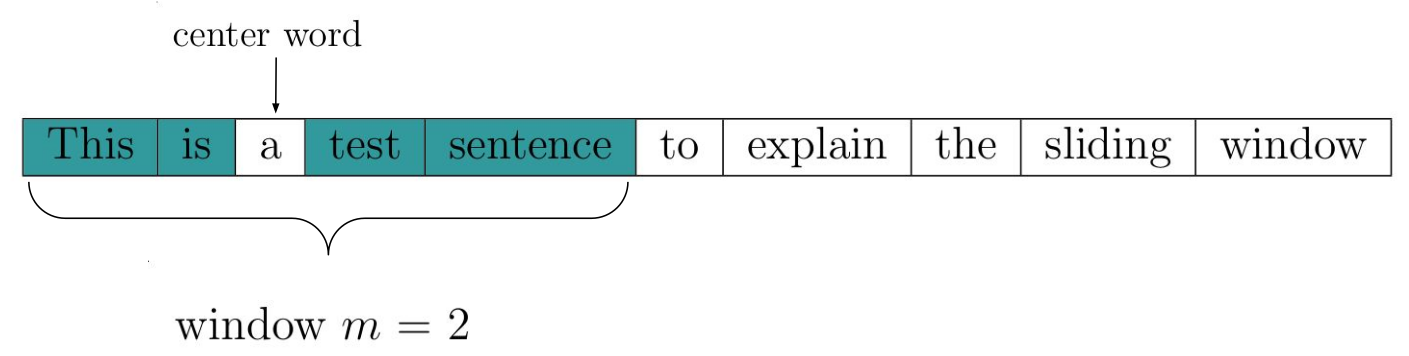
\includegraphics[scale=0.3]{images/window_ex} 
    \caption{Example of a center word and it's context words}
    \label{fig:window_ex}
\end{figure}
%TODO think about example matrix
With these definitions the fake task can be defined: given a pair of center and context words, which will be our training samples, the goal of the network is to predict the probability of each word to appear in the context of the center word.  One may ask how such a network is built. The network consists of two matrices, a projection and an output layer. Both of these matrices store word embeddings. The first one, the projection layer, will store the WE for one specific word in one specific row . It will have dimension $T\times d$, with $T$ being the size of our vocabulary and $d$ the dimension of our WE. The second layer, the output layer, will store one WE in each column. The idea behind these 2 layers is that the input layer will represent our words as center word and the output layer as context words. The task of the network being to predict the probability of each word appearing in the context of a given center word, the following probability should be maximized:\\
\begin{equation} \label{eq:basicSkip}
 \prod_{t=1}^T \prod_{-m<j<m}  p(w_{t+j}|w_t)
 \end{equation}
 Where T is the number of words in the corpus data, $w_t$ the $t^{th}$ word in the corpus data and $m$ is the context window. This means that the $m$ nearest words to $w$ are considered as context words.
Equation \ref{eq:basicSkip} can be transformed into sums by using log probabilities: 
\begin{equation}
 \sum _{t=1}^T \sum_{-m<j<m} log( p(w_{t+j}|w_t) )
\end{equation}
    where the parameters are the same as in Equation \ref{eq:basicSkip}.

The basic Skip-Gram Model uses a classical Softmax to calculate the conditional probability $p(w_{t+j}|w_t)$: 
   \begin{equation} \label{eq:softmax}
   p(w_{t+j}|w_t)=  \frac{exp( \tilde{v}_{w_{t+j}}^Tv_{w_t})}{\sum_{w=1}^v exp(\tilde{v}_w^Tv_{ w_t})}
   \end{equation}
  
  Here $\tilde{v}_{w_t}$ and $ v_{w_t}$ are the vector representations, stored respectively in the projection Layer (first Matrix) and in the output layer (second Matrix). There is a problem with the classical softmax. As a matter of fact, it is unsuitable to compute the softmax. For the computation of $\sum_{w=1}^v exp(\tilde{v_w}^T w_t)$, the denominator in Equation \ref{eq:softmax}, one has to go over the whole corpus data. As very big data sets are needed to train the model, this is not a solution. Mikolov et al. \cite{mikolov2} porposed different solutions. The first solution is to use a Hierarchical softmax introduced by Morin and Bengio \cite{hsoftmax}. In this model, the probability distribution of the output nodes is saved in a binary tree which gives one a logarithmic computation time for each of these probabilities and makes it suitable to compute the softmax. Another possibility is the use of negative sampling which is discussed in the next section.

\section{Negative Sampling}
A second alternative solution to the use of a classical softmax is negative sampling. Negative Sampling is a simplification of Noise Contrastive Estimation (NCE) which was introduced by Gutmann and Hyv{\"a}rinen \cite{nce-original},  and first applied to NLP by Mnih and Teh \cite{mnih}. This section will shortly describe NCE and then how Mikolov et al. \cite{mikolov2} simplified it to create the technique called negative sampling. \\ The idea behind NCE is to distinguish data from noise. It does so by reducing the problem to a logistic regression task and does it by maximizing the log probability. The SGM is only interested in good word representation, hence the probability of the word is not meaningful as long as the quality of the word representations remains high. Mikolov et al. \cite{mikolov2} simplified NCE and called it Negative Sampling, which will be explained next.\\
The main goal of negative sampling is to only update the output nodes of certain words. This will obviously save an enormous amount of computation time. The idea is that given a pair $(c,w) \in D$, where $c$ is a word in the context window of $w$ we select $K$ random words $k_i$ from the corpus data $D$baut. We assume those words do not appear in the context of $w$. We  denote the score that the $(c,w)$ wasn't drawn at random the following way: $p(y=1|c,w)$, and if $(k,w) $ is chosen at random this way: $p(y=0|k,w)$.  Now we use logistic regression to update the weights of the $k$ selected context words and $c$. By doing so we will only have to update $k+1$ nodes.

Let's look at how we construct our objective function for a given word $w$ and one of its context words $c$: 

\begin{align*}
p(c|w) &= p(y=1|c,w) + \prod_{k\in K} p(y=0|k,c) 
\\&= p(y=1|c,w) + \prod_{k\in K} 1- p(y=1|k,c) 
\\&= log((p(y=1|c,w)) + \sum_{k\in K} log(1- p(y=1|k,c)) 
\\&=  log(\frac{1}{1+e^{-v_c \tilde{v_w }}})  + \sum_{k\in K} log(1-\frac{1}{1+e^{-v_c \tilde{v_k}}}) 
\\&=  log(\frac{1}{1+e^{-v_c \tilde{v_w } }})  + \sum_{k\in K} log(\frac{1}{1+e^{v_c \tilde{v_k} }})
\\&= log(\sigma(v_c \tilde{v_w } ) + \sum_{k\in K} \sigma(log(-v_c \tilde{v_k} )) &&\text{where, $\sigma(x) = \frac{1}{1+e^{-x}}$}
\end{align*}\label{eq:obj_neg_samples}

Where $v_c$ and $\tilde{v_w }$, can be interpreted as before in Equation \ref{eq:softmax}. The goal is know to maximize this objective function. Another way too look at this function, apart from logistic regression, and understand why it's working so well, is to assume that two vectors are similar if their dot product is high. Therefore we maximize the dot product of similar words $(w,c)$ ($c$ appears in the context of $w$) and minimize it for dissimilar words $(w,k_i)$ (those were selected randomly).
We see that to compute our objective function we will only have to compute the sum over the number of negative samples $K$. Which, is verys small in practice (2-20). To put things in perspective lets imagine our data set consists of 100000 words, we set $K=2$. Assume each output neuron has a weight vector $v$ with $|v| = 300$. When updating our weights we would only update  $0.2*10^{-2}$ of the 300 million weights in the output layer. 

One question remains: how do we choose our random words? Mikolov et al. \cite{mikolov2} used the following unigram distribution:
 
 \begin{equation} \label{eq:unigram}
P(w)=\frac{f(w)^{\frac{3}{4}}}{\sum_{t=0}^{T} f(w_t)^{\frac{3}{4}}}
\end{equation}
where $f(w)$ is the frequency of $w_t$. The value of $\frac{3}{4}$ is set empirically. Raising the unigram distribution to power of $\frac{3}{4}$ makes it less likelier for a word to be drawn if it appears often in the dataset in comparison to the basic unigram distribution.  See figure \ref{fig:frequency_ex} for an example.
\begin{figure}[ht]
    \centering
            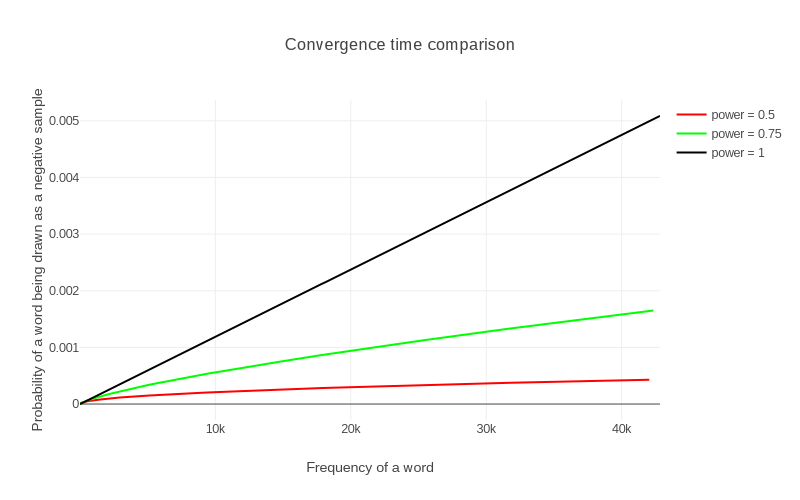
\includegraphics[scale=0.45]{images/frequency_ex} 
    \caption{Probabililty of a word, of the text8 dataset (sampled),  to be chosen at random according to its frequency and the power to which the unigram distribution is raised}
    \label{fig:frequency_ex}
\end{figure}
It's quite easily observable that this approach will outperform the classical softmax in computation time, as it only compute the sum over $K$ output nodes. Now the question arises if the accuracy is good enough but according to Mikolov et al. \cite{mikolov2} the negative sampling method "is an extremely simple training method that learns accurate representations". As a matter of fact, Mikolov et al. \cite{mikolov2} reported a 6\% accuracy improvement in comparison to a Hierarchical Softmax model. Therefore it is a good solution to the problem raised by the classical softmax. 
We now have enough background knowledge about the SGM to look at how it can be optimized. The next section introduces earlier approaches to optimize the SGM.

\section{Optimization of the Skip Gram Model}
Due to the popularity of the SGM, a lot of research went into optimizing it. This research can be divided into two categories, optimization of the throughput and the optimization of the algorithms accuracy. The latter was achieved by allowing words to have multiple meanings, also called context-sensitive word embedings. For our work, the optimization of the throughput is of big interest while the semantic optimization is aimed at giving the reader a more holistic comprehension of the possible research directions. 
This section will first give an overview of the optimization of the throughput and then present one paper that focused on context-sensitive word embeddings. 

\subsection{Optimization of the throughput}

In the original model, the optimization is done with Stochastic Gradient Descent (SGD), which is a sequential algorithm. This process does not favor parallelization. To deal with this specific problem Mikolov et al.\cite{mikolov2} used a Hogwild tree proposed by Recht et al.\cite{hogwild}. The approach is to allow multiple threads to access a shared memory, in this case, the single model. In the original SGM, the threads are constructed as follows: at the beginning of training, the dataset is split into $N$ evenly sized chunks and each of these chunks will be processed by a one thread. The threads run parallelly and have access to the shared memory. Therefore overwriting errors are bound to happen. According to Recht et al.\cite{hogwild} the overwriting errors won't lead to a significant accuracy loss if the data is sparse enough. But in the case of NLP, the problem seems to be a bit more significant, and especially for word embedding, as many words share the same context words. There were several attempts at solving this issue, and we are going to cover a few of them in the following subsections. 

\subsubsection{Parallelization by the use of caching}
This idea was proposed by Vuurens et al. \cite{efficient}. The architecture used here is the basic skip gram model with a hierarchical softmax.  The general idea is to cache the most frequently used nodes of the binary tree used to memorize the probability distribution and update them on the shared single model after a certain number of seen words (the paper used the number 10). The paper produced interesting results as they managed to decrease execution time by increasing the number of cores used for the calculation. This is very powerful because in the original implementation the execution time regressed after using more than 8 cores. It seems to indicate that too much overwriting was happening, as the number of concurrent threads surpasses a certain threshold. This can be seen in Figure \ref{fig:efficient}, where c31 is the model proposed by Vuurens et al.\cite{efficient}. The model did not suffer any accuracy loss in comparison to the original SGM model. 
\begin{figure}[ht]
    \centering
            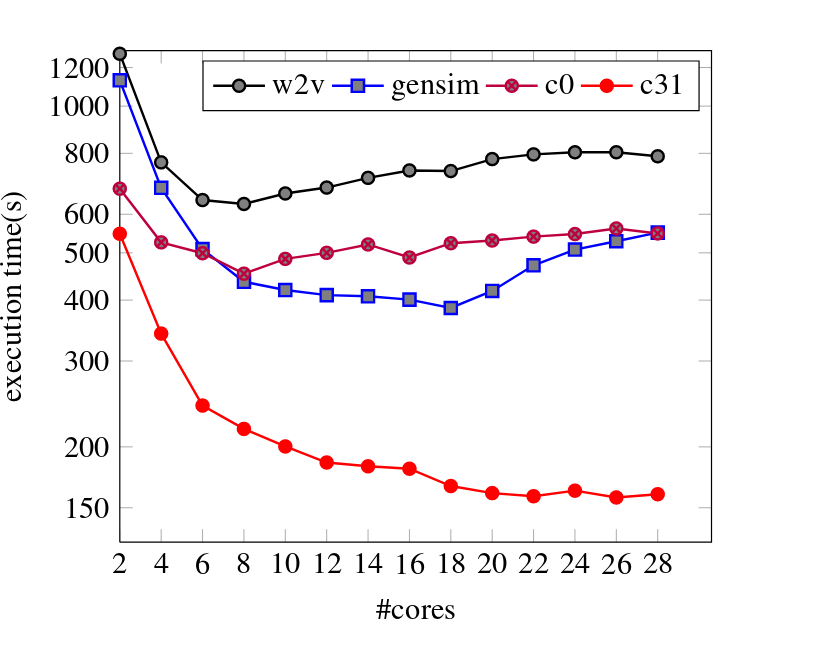
\includegraphics[scale=0.3]{images/cachingEfficiency.png} 
    \caption{Comparasion of the execution time in relation to the number of used cores \cite{efficient}}
    \label{fig:efficient}
\end{figure}
This work proposes a very good way to parallelize the SGM, as in particular, it allows to use more cores during the computation.  As this approached focused on the Hierarchical softmax, in contrast to our work which used negative sampling, the next section covers optimizations of the Skip-Gram Model with negative sampling(SGNS). 

\subsubsection{Parallization in shared and Distributed Memory}
The first parallelized solution which was proposed by Ji et al. \cite{intel}, is to try to reduce the cost of our vector multiplication. The main idea in this paper is to convert the level 1-BLAS (Basic linear subprogram) vector to vector operations to a level 3-BLAS matrix multiplication operation, which are efficiently implemented into hardware and consequently faster. This is achieved, by using the same negative samples for each context word of a given word $w$. Instead of using for each context word a vector to vector multiplication we can transform this into a matrix multiplication, under the assumption that we will not lose accuracy by sharing the same negative samples. The matrix multiplication can be represented in the following way.
\[
\begin{bmatrix}
w \\
w_{n_1}  \\
\vdots \\
w_{n_k}\\
\end{bmatrix}
*
\begin{bmatrix}
w_{c_1}\\
\vdots\\
w_{c_{2m}}\\
\end{bmatrix}
\]

where $w$ is our given word, $w_{n_1}...w_{n_k}$ are the shared negative samples, with $k \in [5,20]$, and $w_{c_1}...w_{c_2m}$ are the words inside of the context window $m$ of $w$, with $m \in [10,20]$, also called a batch of input context words. After each batch the model updates the weights of the used vectors. 
This model achieves a 3.6 fold increase in throughput, by only losing 1\% of accuracy.  An aspect that is not as useful to us is that the experiments were done on CPU, as modern GPU's are often used in many machine learning libraries, as with CUDA for example, there still need work to be done to optimize it with GPU's. This was done by Seulki and Youngmin  \cite{gpu}, which is described in the next section.


\subsubsection{Accelleration of word2vec by Using GPU's}
Seulki and Youngmin  \cite{gpu} focused on getting a better throughput on the SGM when using GPU's. As the SGM is a sequential algorithm, is is not easy to parallelize it, especially if one wants to parallelize the training of individual training samples. As the algorithm goes sequentially over a sentence,  the samples next to each other, in order of execution, will almost every time have the same input word. Therefore it's very hard to parallelize at this level.  To solve this problem, Seulki and Youngmin \cite{gpu} proposed the idea to parallelize the update of each dimension of the word embedding, since those are completely independent of each other. They achieved this by mapping each dimension to a CUDA thread while mapping each sentence to a CUDA block. As each CUDA block runs independently, the training of the sentences is parallelized, and the fact that sentences have different length is of no problem. If the execution time of the GPU kernel is greater than time used to read the sentences, it could be a smart choice to use multiple GPU's. According to Seulki and Youngmin \cite{gpu}, if multiple GPU's are used, there is a need for synchronizing the model, which will hinder run time performance. They achieved their best results with 2 concurrent GPU'S. The accomplished results were very good  as they managed a 20x speedup compared to a single threaded CPU execution, which is a 3x increase in comparison to the original C code from Mikolov et al. \cite{mikolov2}, with no loss in accuracy.  The problem with this and all the above optimization is that the code is not easily available. Therefore we need an optimized implementation of the SGM that is easily available. This is provided by Gensim \cite{gensim}, which will be outlined in the next section.
%%%%%%%%%%%
\subsubsection{Gensim}
Gensim \cite{gensim} is a pure Python library that holds a state of the art implementation of the SGM. Gensim is written in Cython, which first allowed Gensim to have the same runtime as the original C code. Furthermore, it made us of BLAS's and precomputed sigmoid tables, while also trying to parallelize the training of different sentences. This finally yielded in a 4x speedup in runtime.  Gensim is an important tool as it allows us, as a python library, to compare our data rather easily. It was also used in related work \cite{intel} and is therefore of value, as it allows to us compare our work in a simplier way. This concludes our overview of the optimizations of the throughput of the SGM. In the next section, we give a quick outlook of what has been done in the field of context-sensitive word embeddings.



\subsection{Context sensitive word embedding}
A word  has different meanings dependant on its context. This is a problem that is not addressed by the SGM. Some new models, that have taken this issue into consideration, were proposed. A lot of work has been done in this direction, Liu et al.\cite{topicalWE} and Bartunov et al.\cite{breaking} for example, but the one reporting the best results is Liu et al. \cite{contextWithTensor}. The concept of this approach is to change the way we compute the objective function and variables we use in our conditional probability. The idea is to look if a word given a certain context word matches to a topic. \textit{Bank} would match to \textit{finance} given the context word \textit{money}. \textit{Bank} would also match to \textit{nature} if \textit{river} was the given context word. But \textit{Bank} would not match to \textit{nature} with the context word \textit{money} Now one could ask how to achieve such a context sensitive word embedding? First, we have to introduce new variables, therefore let's look at the objective function used: 
\begin{equation}
J(\Omega) = \sum_{(w,t,c)\in D} \sum_{(w,\tilde{t},\tilde{c} \in{\tilde{D}})} max(0,1- g(w,t,c) + g(w,\tilde{t},\tilde{c})) \lambda||\Omega||_{2}^2
\end{equation}

This approach uses the same negative sample technique as described in the previous sections, $D$ is the corpus data and $\tilde{D}$ is the set of negative samples and $\lambda$is the hyperparameter used for the standard $L_2$ standardization. What is interesting here is the function $g(w,c,t)$, where $w$ is a word, $c$ the context word, and $t$ the context in which the word appears. $g$ is defined as follows: 
\begin{equation}
g(w,c,t) = u^T \sigma(w^TM^{[1:k]}t+V_c^T(w \oplus t) + b_c)
\end{equation}
where, $u, V_c, b_c$ are standard parameters for a neural network. $\oplus$ is the vector concatenation. The most important parameter is $M^{[1:k]}$, which is a tensor layer, the tensor layer is used because of its ability to model multiple interactions in the data, as this will be useful for multiple contexts. They used SGD for the optimization of this objective function. They achieved really interesting results as shown in \ref{fig:multipleContext}.\\
\begin{figure}[ht]
    \centering
            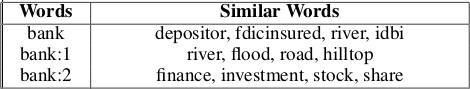
\includegraphics[scale=0.7]{images/multipleContext.png} 
    \caption{"Nearest neighbor words model and Skip-
Gram. The first line in each block is the results of Skip-Gram;
and the rest lines are the results of our model" \cite{contextWithTensor}}
    \label{fig:multipleContext}
\end{figure}

 This will conclude our overview of the related work. We will now give the reader an outline of the different Gradient Descent Optimizer used in our experiments.


\section{Gradient Descent Optimizers} \label{optimizers}
The goal of learning in machine learning is to minimize an objective function  $J(\theta)$, where $\theta$ is the set of all parameters in our model. This happens by updating the parameters $\theta$ at every training time step $t$. We will denote $\theta_{t}$ as the parameters of our model at the $t^{th}$ time step. In this work, we only examine gradient descent algorithms.
\subsection{Gradient Descent}
The idea in gradient descent optimization is to follow the path of steepest descent in the shape of the objective function. To get information about the shape of the objective function, one has to compute the gradients of all our parameters   $\nabla J(\theta_{t})$, where $J$ is our objective function, and $\theta$ all of our parameters, $t$ denotes the time step at which the parameters are taken. We will define $g_{t}$ as the gradients of our parameters $\theta_t$ according to our objective function $J$. To follow the path of steepest descent we will have to subtract a portion of this term from our parameter. The magnitude of the portion is often referred to as the learning rate, denoted as $\eta$. For illustration, this means that the gradients will give the direction of the optimization step, whereas the learning rate will give the amplitude of that step. An update at time step $t$ will result in the following equation:
\begin{equation}
\theta_t = \theta_{t-1} - \eta g_{t-1}
\end{equation}
Where all the variables can be interpreted as above. This will also be the case for further Equations. 
There are three main variations of Gradient Descent, they differ at the moment they chose to update the parameters.
\subsubsection{Stochastic Gradient Descent (SGD)} 
In this variant, the model will update the parameters after each training sample. The problem with this approach is that the variance of the direction of the training step will be very high, as each sample will influence the step individually.

\subsubsection{Batch Gradient Descent} 
Here the update of the model happens after having gone through the entire dataset. The problem with this approach is that one updates the model way to infrequently which will lead to a high convergence time.
\subsubsection{Mini-Batch Gradient Descent} 
Here on updates the model after having gone through a specific number of training samples. The idea is that the batch will be representative of the entire dataset, which will allow the model to learn quicker, as the updates are more frequent (in comparison to batch gradient descent) and less variant (in comparison to SGD).

\subsubsection{Problems with Gradient Descent Algorithms}
SGD, though it's simplicity, is very limited, therefore some issues appear:

\begin{itemize}
\item The learning parameter is yet another hyperparameter to tune, as the optimum setting will largely vary depending on the training task and architecture of the network
\item Learning rate schedules, that diminish the learning rate as the training progresses, are a commonly accepted technique to improve accuracy. This schedule is most often set at the beginning of the training and will be completely independent of the training set. 
\item Every parameter has the same learning rate
\end{itemize}
To tackle those issues numerous advanced optimizers were developed. They will be covered in the next sections. 

\subsection{Momentum}
Momentum is a technique used to address one of SGD weak points. As a matter of fact, because SGD can have trouble computing the optimum of objective function that is only steep in one direction. The problem here is that SGD often oscillates in the direction that is not very steep, and only takes small steps in the steep direction. This issue is addressed by SGD with momentum. 

It does so by adding a percentage of the last update vector to the current update vector. By doing so the gradient that goes in the same direction will get bigger (building momentum) and gradients that go in different directions will annul themselves. 
 At the update $t$ we will comppute our update vector $v_t$ the following way:
\begin{equation}
v_t = \gamma v_{t-1} + \eta \nabla J (\theta)
\end{equation}\label{eq:momentum}
Where $v_t$ and $v_{t-1}$, respectively are the current and the last update vector, and $\gamma$ a hyper parameter, usually set to $0.9$, that defines the importance of the momentum term. We then update our weights as usual: $\theta_t = \theta_{t-1} - v_t$ 
\subsection{Nesterov}
Momentum can be a powerful tool, but sometimes be its own enemy. With Momentum, the learning algorithm often overshoots and blows by the  Optima. Hence it will never converge. This problem was addressed by Yurii Nesterov \cite{nesterov}. The idea behind his algorithm is to incorporate the momentum in the computation of our gradients. We will subtract the previous update vector, or just a fraction,  from our parameters before computing the gradients. Therefore we will compute the gradients of the position where we would be with momentum, which will allow us to make a step in a better direction. The computation of the update vector will look the following way:
\begin{equation}
v_t = \gamma v_{t-1} + \eta \nabla J (\theta -  \gamma v_{t-1})
\end{equation}

Where the parameters as the same used with momentum in equation \ref{eq:momentum}. SGD with momentum and Nesterov accelerated gradient (NAG) has shown tremendous results in RNN's. But some of the earlier mentioned problems still remain.  NAG, still treats every parameter the same way. Therefore we need a more complex optimization algorithm, that takes the frequency of a feature into account. Adagrad does just that. 

\subsection{Adagrad}\label{ssec:adagrad}
Adagrad \cite{adagrad} is an optimizer that tries to apply different learning rates to different parameters, according to their frequency. The idea is to give very frequent features a small learning rate, and very sparse features a high learning rate. This can be very important for our task of word embeddings, as rare words in the corpus are more important than very frequent ones. As a matter of fact, Pennigton et al. used this algorithm for their training of Glove  \cite{glove}, another word embedding system. \\
Each parameter $\theta_i$, at time step $t$ will have it's own learning rate $\eta_{t,i}$
 \begin{equation}
\eta_{t,i} = \frac{\eta_0}{\sqrt{\sum^{t}_{i=1} g^{2}_{t,i}} \epsilon}
\end{equation}
where$g_{t,i} = \nabla J(\theta_{t,i})$  is the partial derivative of the loss function with respect to the parameter $\theta_i$ at time step $t$, and $\epsilon$ is a smoothing factor, so that one does not divide by $0$, at the beginning of the computation and $\eta_0$ is the global learning rate.\\ We see that each parameter $\theta_{i}$ has it's one learning rate. For a very frequent feature the sum of the previous square gradients will be very high, hence the learning rate low. This is how Adagrad achieves a different learning rate for each feature. 
Therefore we have $ \theta_{t,i} = \theta_{t-1,i} - \eta_{t-1,i} g_{t-1,i} $, and we can now construct our global parameter update as follows: 
\begin{equation}
\theta_{t,i} = \theta_{t-1,i}- \frac{\eta}{\sqrt{G_{{t-1}_{i,i}}} + \epsilon} g_{t-1,i}, 
\end{equation} 

with  $G_{t_{i,i}}$ being the diagonal Matrix of the sum of the squares of the graditents ($g_{t,i}^2 $). 
There lies one weakness in this approach: the sum of the squares of the previous gradients grows constantly. This means that after a certain number of epochs the learning rate will be insufficient, to update the model. This issue was addressed by the Adadelta algorithm, that will be covered in the next session. 

\subsection{Adadelta}\label{ssec:adadelta}
Adadelta \cite{adadelta} not only solves the constantly growing sum problem, but also the fact that one does not have to tune the learning rate by not having one. The gist of Adadelta is that instead of taking all the gradients to compute the sum we will only take a fixed number $w$ of gradients. But instead of inefficiently storing w gradients we will take the exponentially decaying average of the squared gradient, denoted $E[g^{2}]$. The average at time step $t$ will be computed in the following way: 
\begin{equation}
E[g^2]_t = \gamma E[g^2]_{t-1} + (1 - \gamma) g^2_t
\end{equation}
where $\gamma$ is a hyperparameter similar to the one used in momentum, that decides how much the past is weighted in contrast to the current gradient. Since Adadelta is an extension of Adagrad the square root of $E[g^{2}]$ is needed which become the Root Mean Squared (RMS) Error:
\begin{equation}
RMS[g]_t = \sqrt{E[g^2]_t + \epsilon}
\end{equation}
Which gives us the following update rule: 
\begin{equation}
\theta_t = \theta_{t-1} - \frac{\eta}{RMS[g]_t}g_t
\end{equation}
Here we have two problems, first, the learning rate is still a hyperparameter. And the units do not match. This is a problem Mathew Zeiler wanted to address. That if the parameters would have units the update parameters units would match. 
Therefore they define the exponentially decaying average of squared parameter updates: 
\begin{equation}
E[\Delta \theta^2]_t = \gamma E[\Delta \theta^2]_{t-1} + (1 - \gamma) \Delta \theta^2_t \ \ \ \ \ \ \hfill \text{,where } \Delta \theta = - \frac{\eta}{RMS[g]_t}g_t
\end{equation}
As before we can know us the root mean squared error: 
\begin{equation}
RMS[\Delta \theta]_{t} = \sqrt{E[\Delta \theta^2]_t + \epsilon}
\end{equation}
As at time step $t$ $RMS[\Delta \theta]_{t} $ is unknown, we approximate it with $ RMS[\Delta \theta]_{t}-1$. Know we replace $\eta$ with  $ RMS[\Delta \theta]_{t}-1$ and get the final update rule: 
\begin{equation}
 \theta_{t+1} = \theta_t - \dfrac{RMS[\Delta \theta]_{t-1}}{RMS[g]_{t}} g_{t}
\end{equation}
\subsection{Adam}
Adaptive Moment Estimation (Adam) \cite{adam}, is a more recent optimization algorithm. It also computes adaptive learning rates. In comparison to Adagrad and Adadelta, it does not only take into considaration the decaying average of the previous squared gradients but also the decaying average of the past gradients. 
Let's introduce : 
\begin{equation}
m_t = \beta_1 m_{t-1} + (1- \beta_1) g_t 
\end{equation}
as the decaying average of the previous gradients, with $\beta_1$ being a hyperparameter similar to $\gamma$ in the previous optimizers,  and 
\begin{equation}
v_t = \beta_2 v_{t-1} + (1- \beta_2) g^2_t 
\end{equation}
 as the decaying average of the previous squared gradients, with $\beta_2$ having the same role as $\beta_1$ \\
One problem arises when using this formula, $m_t$  and $tv_t$ are initialized as vectors of zero. Therefore they are biased towards zero. Therefore a bias corrected version was introduced:\\
\begin{equation}
\tilde{m_t} = \frac{m_t}{1-\beta^t_1}
\end{equation}
\begin{equation}
\tilde{v_t} = \frac{v_t}{1-\beta^t_2}
\end{equation}
The general update is done exactly in the same way as in Adadelta:
\begin{equation}
\theta_{t} = \theta_{t-1} - \frac{\eta}{\tilde{v_{-1}}+ \epsilon} \tilde{m_{t-1}}
\end{equation}
with $\epsilon$ as a smoothing factor and $\eta$ as the global learning rate.  This concludes our overview of gradient descent optimizers, and more generally our background chapter. In the next chapter the reader will be given an outline of our implementation of the Skip-Gram Model.
%\chapter{Research Questions}\label{chap:questions}

This paper will address the following questions: 
\begin{enumerate}
\item Can the convergence time of the skip Gram Model be optimized by the use of advanced optimizers, while at the same time maintaining it's accuracy? 
\item Can the convergence time of the skip Gram Model be optimized by the use of input shuffling, while at the same time maintaining it's accuracy? 
\end{enumerate}


%include{chapters/projectPlan}
\chapter{Methods}\label{chap:methods}
Describe the method/software/tool/algorithm you have developed here

We developped a  full replication of the original w2vec implementation of the Skip Gram Model in Pytorch. And then tried to optimize it. This chapter will illustrate our proceeding. First it will give a short introduction to PyTorch, and then cover the most interesting parts of our implementation. 
\section{PyTorch}
For our implementation we choosed the open source library PyTorch. It offers a few  implementation features that enormlhy facilitates the implemenatation process. First of all it computes the gradient of the loss function online, therofore there is no need for us to implement the calcluation of htose gradients. For the learning ew will only have to use the already implemented optimizers, that can be found in the module torch.optim. Another feature of Pytorch that we used are the classes dataset and dataloader. Both of these classes works closely together.   
\section{Implementation}
\subsection{class SkipGramModel}
This class is responsable for the forward pass of our data, and represents the neural network, that will result in the word embeddings. We used the class torch.embeddings to generate our word embedings. This class allows us to give a single integer to the embeding and it will return our embedding.  
\subsubsection{Method forward()}
. We will take as an input a number of word and their context and then use the same negative samples for all of those words. We will create a matrix made out contex words and samples. Create matrix containing all our words. Multiply the two matrices. this will result in a matrix having each score of equation \ref{obj_neg_samples}. And we will then sum all our scores to return our loss. 
Let's examine an example: $(w_1,c_1)(w_2,c_2)(w_3,c_3)$ be our batch. 
Therefore $pos_u = \begin{bmatrix}
w_1 & w_2 & w_3
\end{bmatrix}, pos_v = \begin{bmatrix}
c1\\
c2\\
c3\end{bmatrix}$ and $neg_v = 
\begin{bmatrix}
k_{1,1} & k_{2,1} & k_{3,1}\\
k_{1,2} & k_{2,2} & k_{3,2}\\
k_{1,3} & k_{2,3} & k_{3,3}\\
\end{bmatrix}$\\
 We then concatenate $pos_v$ and $neg_v$, while negating $neg_v$
resulting in: \\
$samples = \begin{bmatrix}
c_1 & -k_{1,1} & -k_{2,1} & - k_{3,1}\\
c_2 &- k_{1,2} & -k_{2,2} & -k_{3,2}\\
c_3 & -k_{1,3} & -k_{2,3}& - k_{3,3}\\
\end{bmatrix}$

We then multiply $pos_u$ and $samples$ resulting in: \\
$scores = \begin{bmatrix}
w_1 \cdot c_1 & -w_1 \cdot k_{1,1} & -w_1 \cdot  k_{2,1} & -w_1 \cdot  k_{3,1}\\
w_2 \cdot c_2 & -w_2 \cdot k_{1,2} & -w_2 \cdot k_{2,2} & k_{3,2}\\
w_3 \cdot c_3 &-w_3 \cdot c_3  k_{1,3} & -w_3 \cdot c_3 k_{2,3}& k_{3,3}\\
\end{bmatrix}$
Finnally we sum up the score and multiply it with minus one to make it a minimizing problem: \\
 $-(\sum_{i=1}^3 w_i \cdot c_i - \sum_{j=0}^3 -w_i \cdot -k_i,j)$
\subsection{class Dataset}
data loader, pairs neg samples etc.
\subsection{class W2Vec}
tst
\subsubsection{method train\_with\_loader}
training



\chapter{Results}\label{chap:results}


%Describe the experimental setup, the used datasets/parameters and the experimental results achieved

This section will give an overview over the used datasets, the used metric to evaluate our models, the configuration of our model and finally the experimental results achieved.

\section{Dataset}\label{sec:dataset}
In this implementation we mainly used the text8 \footnote{http://mattmahoney.net/dc/enwik8.zip} dataset. We chose this dataset for two reasons. First of all it's a very small dataset, more on exact numbers later, that allowed us to do a lot of computations. Secondly this data set was used in a lot of related work (cite gpu, cpu,caching) hence giving us a very good benchmark. The text8 dataset consists of 1702 lines of 1000 words, there is no punctuation. Therefore we had to choose between building arbitrary sentences and keeping the dataset as it is. We chose the first option because it gives us a faster computation time, and did not show any siginificant loss in quality empirically. We chose a sentences length of 20. Furthermore we applied a technique called subsampling that reduces the data set size. 
We needed a second more larger dataset to confrim our results.  We therefore chose the enwik9 dataset\footnote{http://mattmahoney.net/dc/enwik9.zip}.This dataset needed more preprocessing as it's plain html. We therefore used the a preprocessing script.\footnote{http://mattmahoney.net/dc/textdata.html, Appendix A}. We also splitted this dataset in sentences of length 20, and applied subsampling. The next section will give an exmplanation on the sampling process.
 
 
\subsection{Subsampling}
Subsampling is a technique introduced by Mikolov et al. in \cite{mikolov} to reduce the dataset size while at the same time increasing the quality of the dataset, i.e getting better word embeddings. Certain words that appear very frequently in the dataset such as: "the, as, it, of" do not give an intrinsic value to the words that appear in it's context. Therefore the idea of subsampling is to delete such words from the dataset. This will decrease the computation time and should in theory increase the accuracy of the model. The increase in accuracy can also be explained by the fact that words that would not have appeared in the context of each other, may know, because words between have been deleted, do.
Know the question arises, how one chooses to delete a word. Mikolov et al. chose the following equation to compute the deletion of a word $w$ in the data set:
\begin{equation} \label{eq:sampling}
P(w) = 1- \sqrt{{\frac{t}{f(w)}}}
\end{equation}
where $f(w)$ is the frequency of w, and $t$ is a threshold set empirically. (Mikolov et al.)  recommends a value between $0$ and $10^{-5}$, depending on the size of the dataset. We experimented with different values and $10^{-4}$, seemed the most suited. We did this by simply looking at a random set of sentences and humanly judging the results. Stats about subsampling can be found in table \ref{table:treshold}. Examples in figure \ref{fig:treshold_examples}

\begin{table}[h]
\centering
\begin{tabular}{|l|l|l|l|l|l|}
\hline
Sampling Treshhold &  0      &      $ 1^{-1}$&$   1^{-2}$& $1^{-3}     $ &$1^{-4}   $    \\ \hline
Size of Dataset    & 16 mio & 15mio & 11 mio & 8mio & 4 mio \\ \hline
\end{tabular}
\caption{Size of preproccessed text8 dataset according to sampling treshold}
\label{table:treshold}
\end{table}

\begin{figure}
    \centering
    \begin{subfigure}[b]{\textwidth}
        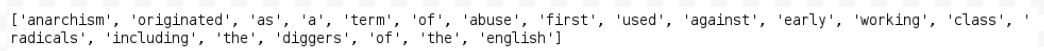
\includegraphics[width=\textwidth]{treshold1}
        \caption{Treshold = $10^{-1}$}
        \label{fig:treshold1}
    \end{subfigure}
    ~ %add desired spacing between images, e. g. ~, \quad, \qquad, \hfill etc. 
      %(or a blank line to force the subfigure onto a new line)
    \begin{subfigure}[b]{\textwidth}
        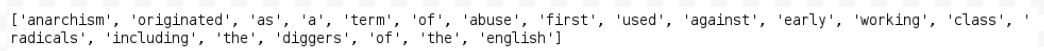
\includegraphics[width=\textwidth]{treshold1}
        \caption{Treshold = $10^{-2}$}
        \label{fig:treshold2}
    \end{subfigure}
    ~ %add desired spacing between images, e. g. ~, \quad, \qquad, \hfill etc. 
    %(or a blank line to force the subfigure onto a new line)
     \begin{subfigure}[b]{\textwidth}
        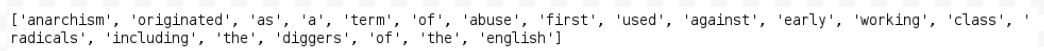
\includegraphics[width=\textwidth]{treshold1}
        \caption{Treshold = $10^{-3}$}
        \label{fig:treshold3}
    \end{subfigure}
   \begin{subfigure}[b]{\textwidth}
        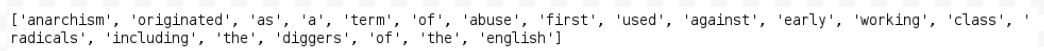
\includegraphics[width=\textwidth]{treshold1}
        \caption{Treshold = $10^{-4}$}
        \label{fig:treshold4}
    \end{subfigure}
     \begin{subfigure}[b]{\textwidth}
        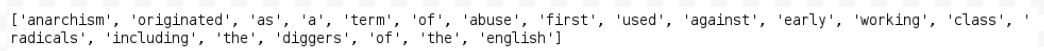
\includegraphics[width=\textwidth]{treshold1}
        \caption{Treshold = $10^{-5}$}
        \label{fig:treshold5}
    \end{subfigure}
    \caption{Example of a sentence with different sampling tresholds}\label{fig:treshold_examples}
\end{figure}

\subsubsection{Min count}
We also applied a threshold in the lower bound, we deleted every word that did not appear more than 5 times in our dataset. We got this tecnique from gensim \cite{gensim}, that introduced this parameter into their training. This is a good technique because of two reasons: first certain words of our data sets do not appear in a common lexicon (twigleg, melqu), or words from a foreign language (gastarbeiter), or names and acronyms. Secondly a word that only appears one time in our dataset will be very dependent on it's original initialization as it will only be updated with it's context pairs. Therefore we applied this technique. It should in theory, such as subsampling, improve the accuracy and  decrease computation time. 

\section{Word similarity}
Evaluating word embedding is not an easy task. We cannot split our data set into train and test set. As the task that the network is learning is of no interest to us. Therefore we need to verify that our embedding are of quality with other techniques. To define quality we first need to define a measure of similarity between two vectors. We will use the cosine distance for this task. The cosine distance of vectors $v$ and $w$ is 1 minus the cosine of the angle between the two vectors. The cosine distance is 0 if two vectors are pointing in the same direction. It's 1 if they are 90 degrees from each other and 2 if they are pointing exactly in the opposite direction. The cosine of the angle between two vectors is calculated by taking the dot product of $v$ and $w$ and dividing it by the magnitude of $v$ and $w$ multiplied with each other. We get then for the cosine distance:
\begin{equation}
cos\_dis(v,w) =1 - \frac{v \cdot w}{|v| |w|} 
\end{equation}

By subtracting 1 from the angle we create a distance between the two vectors, this distance does not take into account any order of magnitude.  Hence for our tasks, two vectors will be considered equal if they are of different magnitude but point in the same direction. 
This technique a part from being shown empirically to work very well to measure the quality of word embedding has another advantage. By normalizing the vectors the calculation of the cosine angle becomes the dot product of the two vectors. Which can be computed very fast on modern gpu's. 

Know that we have a measure to compute the similairty of two vectors let us introduce a way to rate the quality of our embedings.


\subsubsection{wordsim353}
To measure the quality of our word embedding we will need a dataset to compare our results too. We chose  wordsim353\footnote{wordsim353} for this task, as it's the most used in similar literature. The data set consits of 353 pairs of words rated by humans on their similarity. The similarity score is in the range of 1 and 10. See \ref{fig:ws353_ex} for two examples of such pairs. We will rank our embedings on the pearson corelation coefficient between the cosine distance and the scores attributed by humans. 
\begin{figure}[ht]
    \centering
			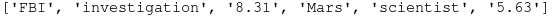
\includegraphics[scale=0.7]{images/wordsim353_example} 
    \caption{Example of pairs and their rating in wordsim353}
    \label{fig:ws353_ex}
\end{figure}

\section{Configuration of the network}
The skip gram model, has a lot of possible options, that can be tuned. We configured one model and then only changed the learning rate. The explanation of the parameters will be structerd as follow: 
\texttt{Parameter} - Description and tuning -  \textit{Value}
\begin{itemize}
\item \texttt{Negative Samples} Here we have to find a trade off between, setting the parameter too high which will result in increased accuracy but a longer computation time. For smaller dataset a higher negative samples is often needed. We experimented early with 5, 10,15 - \textit{10}
\item \texttt{Context Window:} The bigger the window the more training examples the network will have, but if the window is to big the semantic meaning of the window will be erased. Mikolov et al. proposed a setting between 2-10. - \textit{5}
\item\texttt{ Dimension of the embedding}: Here the choice is less obvious, the higher the dimension the better the embedding should be.( cite paper dimension vectors talk about gensim ) but when tested on gensim 100 yielded better results than 300 - \textit{100}
\item \texttt{Batch size}: As described in section FORWARD, there is a trade off to find between accuracy and training time. We first used a batch size of 5000, but then decide after non conclusive results  that 2000 would be better - \textit{2000}
\item \texttt{Alpha}: learnng rate, this hyper parameter was tuned in every optimizer therefore only the range will be indicated - \textit{(1e-5,1)}
\end{itemize}

\section{Input Shuffling}
We used input shuffling as a technique to optimize the skip gram model. We will first describe input shuffling in a general way and then explain why we suppose that input shuffling could work well on the skip gram model. 
Let $X = {x_1...x_n}$ be our input data set. Input Shuffling describes the process of taking a random permutation of the dataset as an input at each epoch. 
The idea behind this technique, is the same as the use of mini batches. We want to present our optimizer with different loss surfaces, so that it's able to find the best optimum. But both combined can be a very powerful, there always lies a risk that a mini-batch isn't a good representative of the true gradient. This way, by shuffling the input, one would avoid this bias.
There are two reasons why we thnik that input shuffling is particulary well suited for the skip gram model. The first one has to do with the fact that when we read our words sequentially that words that only appear very early will not benefit from the context words being already updated from others. The second thing is that we used the special batch technique described in section x.  When using this technique and not using shuffling we will always have words that appear next to each other in a batch and will therefore updat similar words at the same time. We then loose some accuracy. But if instead we would use input shuffling then in one batch the words would likely not be similar and therefore overwriting will be less likely. 
One thing to consider is that when using input shuffling we cannot use a sliding window size. 

\section{Convergence time} 
To optimize convergence time we have to define convergence time first. Therefore we used the already available implementation gensim. we know from \cite{intel}. that a score of $0.66$ in the task of word similarity is the state of the art. We also know after testing Gensim ( more on this process in section discussion), that it takes 4 epochs to converge. Therefore we defined the following criteria for convergence: \\
$\rho - \rho_{prev} < 0.009 \vee or \rho = 0.66$ \\
where $\rho$ is the pearson coefficient with the wordsim353 task. 

\section{Results by optimizer}
We ran multiple experiments for each optimizer. This section will only give an overview over the quantified results. 

\subsection{SGD}
The first challenge for each optimizer was to find a correct learning rate. We first tried the learning rate suggested by gensim, and then performed a random search to find the best one.As expected a bell curve shape resulted, with a learning rate that is to high our model diverged and with a learning rate that is two low or model would not learn quick enough. The best setting that we found is $0.0075$. We converged in 11 epochs. The second experiment was to add input shuffling. 
As seen is figure \ref{fig:results_sgd}, for every learning rate the convergence time decreased. Our model know converges in only 7 epochs. Another intersting point to point out of figure \ref{fig:results_sgd} is that with input shuffling we achieved better results with higher learning rates. As for learning rates of $0.01$ and $0.025$ we did converge in 11 epochs with input shuffling but did not converge in 20 epochs without it.

\begin{figure}[h]
    \centering
			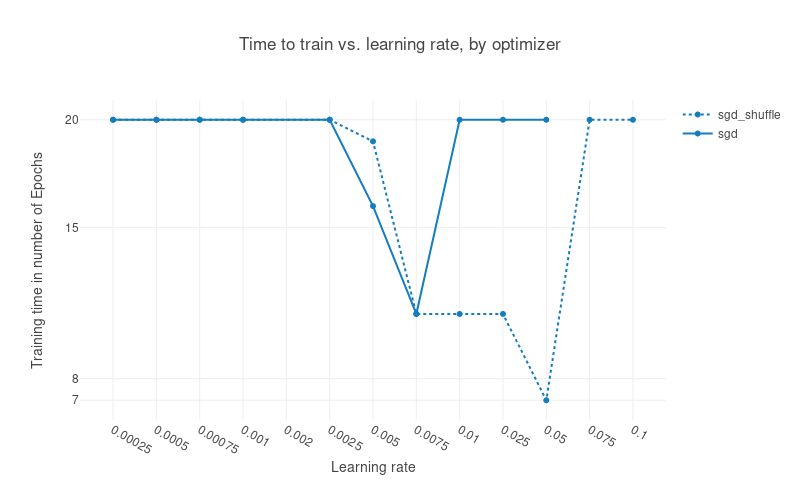
\includegraphics[scale=0.45]{images/results_sgd_shuffle} 
    \caption{Training time Stochastic Gradient Descent with input Shuffling}
    \label{fig:results_sgd}
\end{figure}
\subsection{Momentum and Nesterov}
Momentum and Nesterov accelerated gradient both have an additional hyper parameter $\gamma$, that, as described in Section \ref{optimizers}, defines the percentage of the previous gradient that will be added to the current gradients. We set $\gamma = 0.9$ as this is the typical value, and did not alter it during our experiments. Momentum and Nesterov alone respectively only slightly decrease or increase the convergence time. As the first one optimally converges in 9 epochs and the second one in 13. If we add input shuffling to the equation, interestingly the same things appear as with plain SGD. The convergence time gets better, 8 and 3 epochs until convergence respectively, and higher learning rate do also yield better results. 
\begin{figure}[h]
\centering
\begin{minipage}{.5\textwidth}
  \centering
  	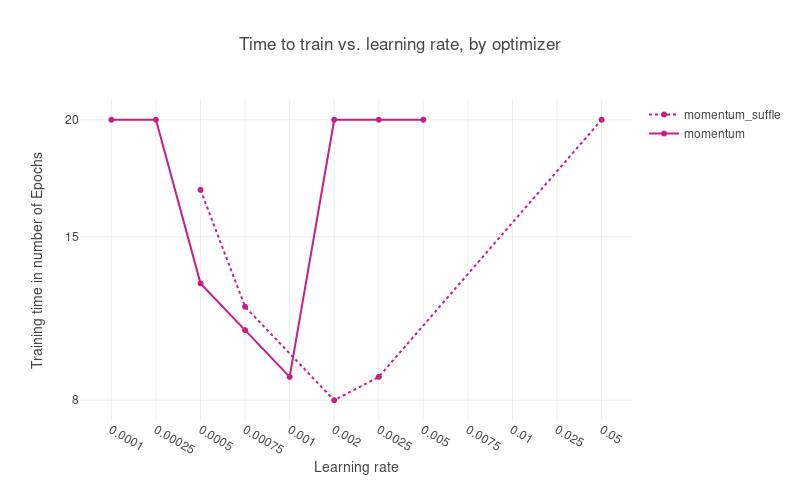
\includegraphics[scale=0.3]{images/results_mom_shuffle} 
    \caption{Training time  Momentum with input Shuffling}
    \label{fig:results_mom}
  \label{fig:test1}
\end{minipage}%
\begin{minipage}{.5\textwidth}
  \centering
	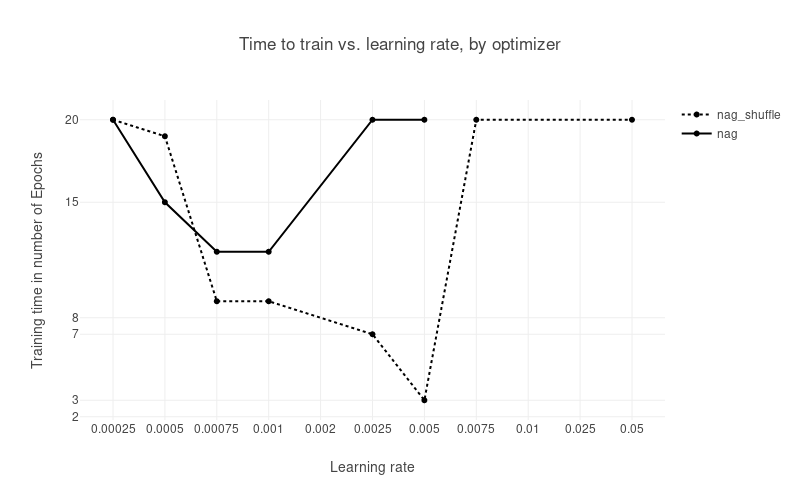
\includegraphics[scale=0.3]{images/results_nag_shuffle} 
    \caption{Training time  Nesterov with input Shuffling}
    \label{fig:results_nag}
\end{minipage}
\end{figure}
\subsection{Adagrad}
Adagrad is a very interesting tool for learning word embedding as they decrease the learning rate for very frequent occuring features, and vice versa for low frequent words. Because words that appear very frequently often do not have a real semantic gain to their context words, it's good to have a low learning rate. So in theory Adagrad is particullary well suited for our task. This was confirmed empirically as our model converged in 4 epochs. When combined with shuffling adagrad only took 3 epochs to converge. This shows the tendency of the skip gram model to converge faster with input shuffling and the big impact of having different learning rate for each feature. 
Here it's interesting to notice that a higher learning rate combined with input shuffling did not yield better results then without shuffling. Both of our best results happened with a learning rate of $0.1$. 
\begin{figure}[h]
    \centering
			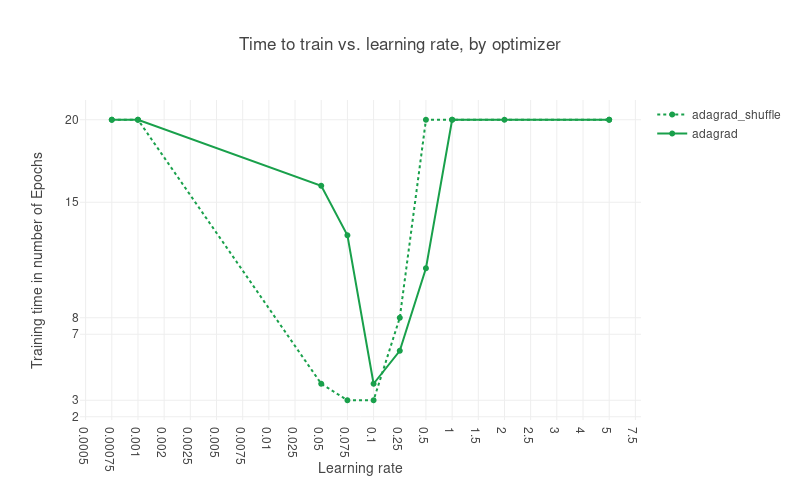
\includegraphics[scale=0.45]{images/results_adagrad_shuffle} 
    \caption{Training time Adagrad with input Shuffling}
    \label{fig:results_adagrad_shuffle}
\end{figure}
\subsection{Adadelta}
In theory Adadelta should outperfrom Adagrad as it's its upgrade. But it did not hold up to our excpectations. Because it didn't has any learning rate to tune, we only did 2 experiments, with and without input shuffling. Adadelta did not manage to achieve a word similarity of 0.66. It only converged to a similarity of 0.59. It did this in 20 epochs without input shuffling and in 3 with input shuffling. As seen in table \ref{table:results_adadelta}
\begin{table}[h]
\centering
\begin{tabular}{|l|l|l|}
\hline
Adadelta Model    & Convergence Time & Word similarity \\ \hline
Without Shuffling & 20               & 0.59            \\ \hline
With Shuffling    & 3                & 0.59            \\ \hline
\end{tabular}
\caption{Convergence Time and Quality with Adadelta}
\label{table:results_adadelta}
\end{table}
\subsection{Adam}
Adam is the most advanced of all the optimizers used in our experiments. Did it therefore yield the best results? Indeed this was the case, as seen in figure \ref{fig:results_adam_shuffle}, Adam converged in 3 epochs without shuffling and 2 with. This are the best result that we got with any optimizer.  It's also intersting to note that as same as with Adagrad it did not react to input shuffling the same way as SGD did. In fact it worked in the opposit direction. We achieved our best result with input shuffling with a lower learning rate $0.001$ then we used to achieve the best result without input shuffling $0.05$
\begin{figure}[h]
    \centering
			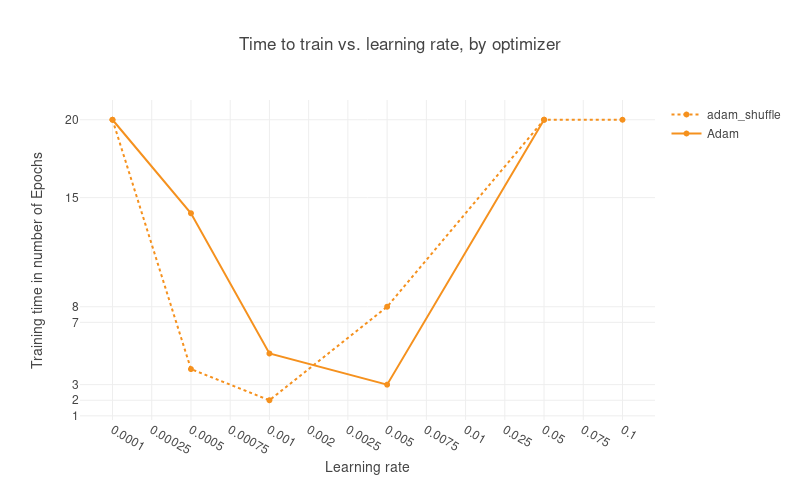
\includegraphics[scale=0.45]{images/results_adam_shuffle} 
    \caption{Training time Adam with input Shuffling}
    \label{fig:results_adam_shuffle}
\end{figure}
\chapter{Discussion}\label{chap:discussion}


%Discuss the results. What is the outcome of your experimetns?

In this secftion we will shortly discuss our results then extensively compare our work to related work, try to make sense out of our results, discuss some challenges faced and finally possible future work. 

\section{Our work}
In this section we will quickly discuss our findings, and try to give some explanation to it.  
\subsection{Shuffling and learning rate with SGD}
As shown in figures \ref{fig:results_sgd}, \ref{fig:results_mom} and \ref{fig:results_nag}, the model, when using SGD as an optimizer,  was able to use a higher learning rate when the input was shuffled as when not. Therefore arises the questions why those this phenomen happen. One possibility is that the model is presented with a slightly different loss function every time, which is closer to the optimal loss function, therefore the steps taken by the optimizer are closer to the optimum and can therefore be bigger. 

\subsubsection{Large differences with nag and sgd when using shuffling}
As swhon in figures \ref{fig:results_sgd} and \ref{fig:results_nag}, plain SGD and Nesterov Accelerated gradient, greatly differ in their convergence time when using shufflin in to comparison when not. We attribute these results partially to a good random initialization guess and not only input shuffling. Due to a lack of time these results where not replicate more then once. 

\section{Related Work}
In this section we will compare - our work to related work, we will first compare us to the baseline model, the original c implementation from Mikolov et al \cite{Mikolov}. We will then compare our self to Gensim, we do this because Gensim allowed us to easily and fastly compute the embeddings, while having access to the loss, and being a python implementaion made everything easier. 

\subsection{word2vec}
%TODO ask jorg

As mikolov et al. published the original paper about which introduced the SGNS, it is of course releveant to compare ourselves to theim. The first important thing to notice is that Mikolov et al. only trained their model on the very large google news dataset incorporating more than 3 billion words. This makes the comparison of our work more problematic and more of a guessing game. But we will make some assumptions, as they can become interesting. 
In their original paper, Mikolov et al. reported results from 1 and 3. We accord these good results to the very large dataset  and furthermore as a matter of fact their result are better with 3 than with 1 epochs. We do not have any informtaion about the convergence. Hence it would be intersting to use their dataset for comparison. \\
One thing we can compare is the quality of our word embeddings. Mikolov et al. did not report any results on their model with the text8 dataset, but they therefore published their code, and Ji et al \cite{intel} tested the model on the text8 dataset. They reported a similarity of 0.63 on the wordsim task. This is obviously outperformed by all our models. We did not find any explanation on why those results differ as much. \\
The final assumption is that an advanced optimizer could maybe outperform Sgd in terms of quality on a large embedding. This will be discussed in further work.
 


\subsection{Gensim}
Gensim does propose the class w2vec with the following possible parameters\footnote{link to gensim params}, we will describe theim, show our setting, and why we chose the following, we will only describe the prametrs we changed from the default value will be explained, the rest can be found in the appendix. 
They will be presented in the following way: \\
\texttt{name} (type) - \textit{Description} - Value
\begin{itemize}

   \item \texttt{sentences} (iterable of iterables) – Dataset - we used the Original text8 document splitted into sentences of length 20
  \item \texttt{ size }(int) – Dimensionality of the word vectors - 100
\item    \texttt{window} (int) – Maximum distance between the current and predicted word within a sentence - 100
  \item  \texttt{min\_count }(int) – Ignores all words with total frequency lower than this - 5
 \item   \texttt{workers} (int) – Use these many worker threads to train the model (=faster training with multicore machines) - 4 
\item    \texttt{sg} ({0, 1}) – Training algorithm: 1 for skip-gram; otherwise CBOW. -1
  \item  \texttt{hs} ({0, 1}) – If 1, hierarchical softmax will be used for model training. If 0, and negative is non-zero, negative sampling will be used. - 0
  \item  \texttt{negative} (int) – If > 0, negative sampling will be used, the int for negative specifies how many “noise words” should be drawn (usually between 5-20). If set to 0, no negative sampling is used - 10 
\item   \texttt{ ns\_exponent} (float) – Exponent in the unigram distribution, when choosing random samples REFERENCE EQUATION. - 0.75
\item    \texttt{alpha} (float) – The initial learning rate. - 0.025
 \item   \texttt{min\_alpha} (float) – Learning rate will linearly drop to min\_alpha as training progresses. -0.0001

 \item   \texttt{sample} (float) – The threshold for configuring which higher-frequency words are randomly downsampled, useful range is (0, 1e-5). - 1e-4
   \item \texttt{hashfxn} (function) – Hash function to use to randomly initialize weights, for increased training reproducibility. - VERIFY 
  \item  \texttt{iter} (int) – Number of iterations (epochs) over the corpus. - 10 
 \
  \item  \texttt{compute\_loss} (bool) – If True, computes and stores loss value which can be retrieved using get\_latest\_training\_loss(). - True
 \item   \texttt{callbacks} (iterable of CallbackAny2Vec) – Sequence of callbacks to be executed at specific stages during training. - see Appendix
\end{itemize}

\subsubsection{Gensim vs. SGD}
First we have to note that we cannot compare ourselves to gensim in computation time, this woudl not be very smart as our code is written in python and gensim uses advanced cython routines\footnote{link to tutorial thesis}. 
The first interesting thing to note is that we did not have the same values in convergence time as gensim when using sgd. There are differnet possiblilities why this could be the case. First our batched approach could hinder performance in term of convergence as some overwriting may happen. Another differnce between our implementation is the fact that gensim checks whether negative samples are real negative samples. Thererfore the learning of the input and output context is optimized. 
The first hypothesis may be confirmed by the fact that our input shuffling reduces the number of overwritings and therefore we achieved conv time of 7 epcohs which is closer to 4 epochs. and the last difference maybe explained by the eg samples thing. 

\subsubsection{Gensim vs. Adam}
The Adam optimizer did outperform the Gensim application in performance (only slighltlly: 0.01 corr coeff advantage) and convergence time. Adam converged in 2 epochs vs. Gensim in 4. The case to be made here is that one would have to look at the computational advantage to calculate the simple sgd vs.  the adam update rule. Another aspect to look at is that we mainly tested our implementation on the text8 dataset. We only experienced once one the enwik9 dataset. Here the argument that can be made is that, some optimizers work better on specific loss functions in comparison to others, hence we need to show that our optimizer words on amultiued on theim and that it is not just a statistical anomaly.

\begin{figure}[h]
    \centering
			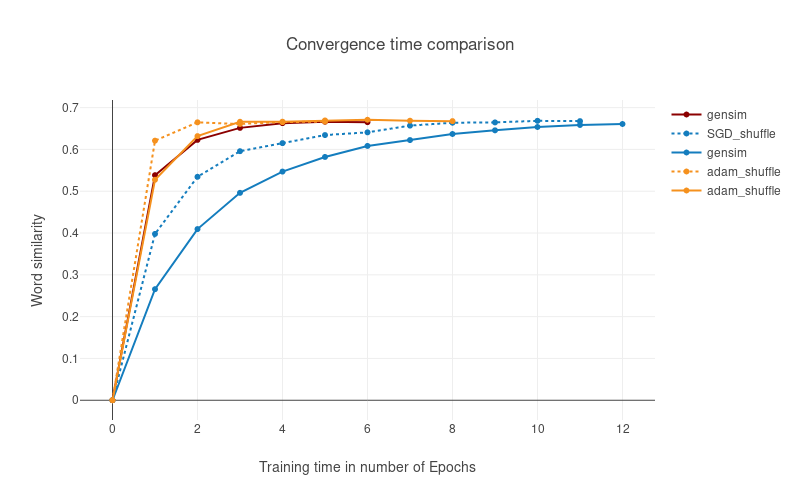
\includegraphics[scale=0.45]{images/gensim_vs_adam} 
    \caption{Training time Stochastic Gradient Descent with input Shuffling}
    \label{fig:gensim_vs_adam}
\end{figure}


\section{Challenges faced}
\subsection{Using the wrong embeddings}
To start our comutation we did choose some wrong, at leat not in coordinance with gensim, initialization embeddings. The context vectors were set between (-1,1) distributed normally. Gensim does it buy putting theim all to 0. As we did the latter the first time our model did not train, but this is possably due to a learning rate that was too low. So we chosed theim to (-1,1). With theim we did not acheive the same similarity as gensim. But when we changed theim back we performed the same results as gensim. Therefore this is a recommendation to future work to not set the initialization to (-1,1)
\subsection{Too big of a batch size}
Another challenge we faced was finding a good batch size. We trained our batch size for a long time with a bs of 5000. But this seemed to worked fine in the beginning but a high lr seemed to work too which was very suspect. We then decided to take a batch size of 2000. Which slightly decreased the learning time, and increased the convergence time and adjusted the learning rate. 
\subsection{Correct loss function}
We expirimented with different loss function as we did not have exactly the same as introduced by mikolov et al. We therefore first ook the average of each score in our tensor. But we then took the sum which seemed to work  better. Is this because the shape of the loss function suits bettter advanced optimizers. Or because it approaches the original loss function more. 


\section{Further Work}
This work only focused on testing the approach of using advanced optimizers and input shuffling to improve the convergence time of the SGNS. While we did show that in theory it could work there dstill needs a bit of work to be done to show that this claim holds consistently. The first thing to do is to use another data set we only tried our approach on only one and a very small dataset. Both of these aspects are problematic. By using a very small dataset we do not use the model in the condition it is mostly needed for as the dataset used in practice a usually 3b words. There is a small argument that can be made for machine translation as the use of small parllel corpus is not unusual . The second one is that some optimizers have shown to perform better on some specific shapes of loss functions. Therefore it could be possible that adam and adagrad only outperform the sgd on this specific loss function for this dataset. Therefore there still needs to be more extensive work done to confirm to confirm our interesting early results. Antoher issue with our implementation is that we didn't care about the throughput of words, so in this matter our implementation is inefficient. One would have to improve one of the already efficient implementation in order to show that we can imporve the convergence time while at the same time maintaining the same convergence time.




\begin{frame}
\frametitle{Conclusion} 
\begin{itemize}
\item Skip Gram Model powerful yet simple tool to create word embedings
\item Advanced optimizers especially Adagrad and Adam improve convergence time 
\item Improved convergence time, while maintaining accuracy
\end{itemize}
\end{frame}

%-- Appendix (optional)
\begin{appendices}
   % !TeX spellcheck = en_US
% !TeX encoding = UTF-8

% Custom colors

% Python style for highlighting

\chapter{Code}
\section{Gensim}
The code used to retrieve information from Gensim computation. 
\lstinputlisting[language=Python]{epoch_logger.py}
 \chapter{Math}

\chapter{Parameters}

\chapter{Dataset}
These are the parameter that we did not alter during the training of Genism:
\begin{itemize}
   \item \texttt{hashfxn} (function) -- \textit{Hash function to use to randomly initialize weights, for increased training reproducibility. }-- VERIFY 
  \item  \texttt{hs} ({0, 1}) --\textit{ If 1, hierarchical softmax will be used for model training. If 0, and negative is non--zero, negative sampling will be used. }-- 0
 \item  \texttt{ corpus\_file} (str, optional) – None
   \item \texttt{cbow}\_mean ({0, 1}, optional) - Unnecessary since cbow is not used
    \item seed (int, optional) – Seed for the random number generator. Initial vectors for each word are seeded with a hash of the concatenation of word + str(seed). Note that for a fully deterministically-reproducible run, you must also limit the model to a single worker thread (workers=1), to eliminate ordering jitter from OS thread scheduling. (In Python 3, reproducibility between interpreter launches also requires use of the PYTHONHASHSEED environment variable to control hash randomization). - None 
\item   \texttt{ max\_vocab\_size} (int, optional) – Limits the RAM during vocabulary building; if there are more unique words than this, then prune the infrequent ones. Every 10 million word types need about 1GB of RAM. Set to None for no limit. - None 
\item \texttt{   max\_final\_vocab} (int, optional) – Limits the vocab to a target vocab size by automatically picking a matching min\_count. If the specified min\_count is more than the calculated min\_count, the specified min\_count will be used. Set to None if not required. - None
item\texttt{   trim\_rule} (function, optional) –Vocabulary trimming rule, specifies whether certain words should remain in the vocabulary, be trimmed away, or handled using the default (discard if word count < min\_count). Can be None (min\_count will be used, look to keep\_vocab\_item()), or a callable that accepts parameters (word, count, min\_count) and returns either gensim.utils.RULE\_DISCARD, gensim.utils.RULE\_KEEP or gensim.utils.RULE\_DEFAULT. The rule, if given, is only used to prune vocabulary during build\_vocab() and is not stored as part of the model.

    The input parameters are of the following types:
            word (str) - the word we are examining
            count (int) - the word’s frequency count in the corpus
            min\_count (int) - the minimum count threshold. - None

  \item  \texttt{sorted\_vocab }({0, 1}, optional) – If 1, sort the vocabulary by descending frequency before assigning word indexes. See sort\_vocab(). - None
 \item   \texttt{batch\_words }(int, optional) – Target size (in words) for batches of examples passed to worker threads (and thus cython routines).(Larger batches will be passed if individual texts are longer than 10000 words, but the standard cython code truncates to that maximum.) - None 
\end{itemize}


 \end{appendices}
\newpage


%%%%%%%%%%%%%%%%%%%%%%%%%%%%%%%%%%%%%%%%%%%%%%%%%%%%%%%%%%%%%%%%%%%%%%%%%%%%%%%%%%%%%%%%%
\backmatter

% -- Bibliography
\printbibliography

% -- Eidesstattliche Erklärung (= Affadavit)
%% !TeX spellcheck = de_DE
% !TeX encoding = UTF-8

\chapter{Eidesstattliche Erkl\"arung}

	Hiermit versichere ich, dass ich diese \thesisType{} selbstst\"andig und ohne Benutzung anderer als der angegebenen Quellen und Hilfsmittel angefertigt habe und alle Ausf\"uhrungen, die w\"ortlich oder sinngem\"a\ss{} übernommen wurden, als solche gekennzeichnet sind, sowie, dass ich die \thesisType ~in gleicher oder \"ahnlicher Form noch keiner anderen Pr\"ufungsbeh\"orde vorgelegt habe.

	\vspace{3cm}

	Passau, \thedate

	\vspace{2cm}

	\parbox{8cm}{
		\hrule \strut \theauthor
	}




\end{document}
